\subsection{Fixed Income Valuation}

\begin{definition} \hlt{Time Value of Money}
\begin{equation}
PV = \sum\limits_{t=1}^N \frac{PMT}{(1+r)^t} + \frac{FV}{(1+r)^N} \nonumber
\end{equation}
where $PV$ is present value of bond, $PMT$ is coupon payment, $FV$ is face value, $r$ is required rate of return.\\
\end{definition}

\begin{definition} \hlt{Yield to Maturity (YTM)}\\
Time value of money equation may be modified to solve for $r$ (internal rate of return on cash flows). This is the implied or observed single market discount rate. Assumes the following:
\begin{enumerate}[label=\roman*.]
\setlength{\itemsep}{0pt}
\item Investor holds bond to maturity
\item All coupon and principal payments are on scheduled dates
\item Investor is able to reinvest coupon payments at the same yield
\end{enumerate}
\end{definition}

\begin{definition} \hlt{Horizon Yield}\\
Internal rate of return between total return and purchase price of bond.\\
The horizon yield on a bond investment is the annualised holding-period rate of return.
\end{definition}

\subsubsection{Pricing of Fixed Income}

\begin{definition} \hlt{Flat Price, Accrued Interest, Full Price}\\
When bond is priced between coupon payment dates, its price has two components: the flat price $PV^{\text{Flat}}$, and the accrued interest $AI$. Sum of the parts is the full price $PV^{\text{Full}}$.
\begin{align}
PV^{\text{Full}} &= PV^{\text{Flat}} + AI \nonumber \\
AI &= \frac{t}{T} \times PMT \nonumber
\end{align}
where $t$ is number of days from prior coupon payment to settlement date, $T$ is number of days in coupon period.
\end{definition}

\begin{figure}[H]
\centering
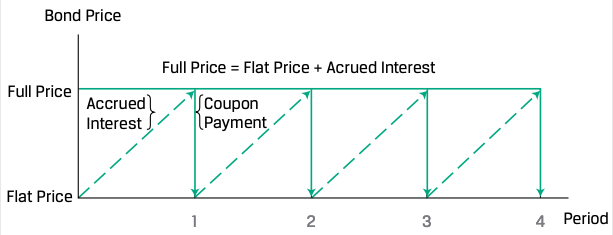
\includegraphics[scale=0.4]{/fi/fullprice}
\caption{Full price of the bond}
\end{figure}

\begin{remark} \hlt{Conventions for Day Counting}\\
Specified by two parameters: how days are counted in a given period, and the number of days assumed per period. Common conventions are $30/360$ and Actual$/$Actual
\end{remark}

\begin{remark} \hlt{Full Price and Payment}\\
Full price of fixed-rate bond between coupon payments, given by market discount rate per period $r$, is present value of future cash flows as of trade settlement ate.
\begin{align}
PV^{\text{Full}} &= \sum\limits_{n=1}^N \frac{PMT}{(1+r)^{n-t/T}} + \frac{FV}{(1+r)^{N-t/T}} \nonumber \\
&= \left[ \sum\limits_{n=1}^N \frac{PMT}{(1+r)^{n}} + \frac{FV}{(1+r)^{N}} \right] \times (1+r)^{t/T} \nonumber \\
&= PV \times (1+r)^{t/T} \nonumber
\end{align}
\end{remark}


\begin{remark} \hlt{Quotation for Bonds}\\
On a basis-point ($100$-point) system, i.e., $@106$ means $106\%$ of face value.\\
If coupon rate $<$ market discount rate, then $PV < 100$, the bond is at a discount.\\
If coupon rate $=$ market discount rate, then $PV = 100$, the bond is at par.\\
If coupon rate $>$ market discount rate, then $PV > 100$, the bond is at a premium.
\end{remark}

\begin{remark} \hlt{Price and Interest Rate Relationship}\\
Bond prices and interest rates are inversely related. Price decreases as interest rate increases.
\end{remark}

\begin{remark} \hlt{Spot Rate Pricing}\\
Spot rate is the yield-to-maturity on zero-coupon bonds.\\
Calculate with sequence of market discount rates corresponding to the CF dates.
\begin{equation}
PV = \sum\limits_{t=1}^N \frac{PMT}{(1+Z_t)^{t}} + \frac{FV}{(1+Z_N)^{N}} \nonumber
\end{equation}
where $Z_t$ is the spot rate/zero-coupon yield for period $t$.
\end{remark}

\begin{remark} \hlt{Bond Relationships}
\begin{enumerate}[label=\roman*.]
\setlength{\itemsep}{0pt}
\item Inverse Relationship: bond prices and interest rates are inversely related.\\
Price decreases as interest rate increases.
\item Convexity Effect: for the same coupon rate and time-to-maturity, $\abs{\% \Delta \text{Price}}_{r \downarrow} > \abs{\% \Delta \text{Price}}_{r \uparrow}$.\\
Prices are more volatile on the upside for a $1\%$ change in interest rate.
\item Coupon Effect: given same time-to-maturity, lower-coupon bond has greater $\% \Delta$ Price than higher-coupon bond for same change in market discount rates.
\item Maturity effect: given same coupon rate, longer-term bond has greater $\% \Delta$ Price than shorter-term bond for same change in market discount rates. May not hold for low-coupon, long-term discount bonds
\end{enumerate}
\end{remark}

\begin{figure}[H]
\centering
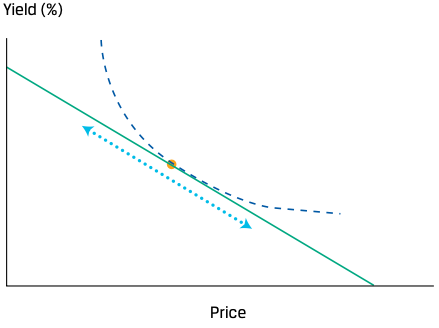
\includegraphics[scale=0.4]{/fi/convexpyrel}
\caption{Convex Price-Yield Relationship}
\end{figure}

\begin{remark} \hlt{Constant-Yield Price Trajectory}\\
As time passes, bondholder comes closer to receiving par value at maturity.\\
Price of bond approaches par value as its time-to-maturity approaches zero.\\
Carrying value is purchase price plus amortised amount of discount if purchased below par value, or minus amortised amount of premium if purchased above par value.
\end{remark}

\begin{figure}[H]
\centering
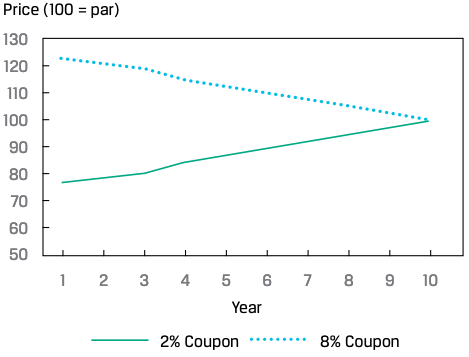
\includegraphics[scale=0.4]{/fi/constpricetraj}
\caption{Constant-Yield Price Trajectory}
\end{figure}

\begin{remark} Purpose of Matrix Pricing\\
To price illiquid or new fixed-rate bonds.\\
Underwriting new bonds to get an estimate of the required yield spread over the benchmark rate.\\
Estimate market discount rate and price based on quoted or flat prices of more frequently traded comparable bonds, with similar time-to-maturity, coupon rates, and credit quality.
\end{remark}

\begin{method} \hlt{Determining Price of New or Illiquid Bond with Matrix Pricing}
\begin{enumerate}[label=\roman*.]
\setlength{\itemsep}{0pt}
\item Identify actively traded, comparable bonds with similar times-to-maturity, coupon rates, credit quality.
\item Calculate YTM for each comparable bonds, and calculate average yield for each maturity year.
\item Linearly interpolate the YTMs of comparable bonds to estimate YTM closest to target bond maturity.
\item Using estimated YTM, calculate price of new/illiquid bond by discounting all coupon and principal.
\end{enumerate}
\end{method}

\begin{figure}[H]
\centering
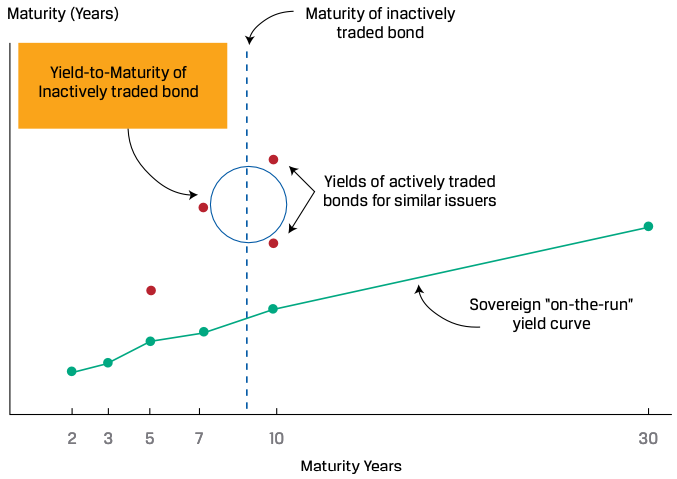
\includegraphics[scale=0.45]{/fi/matrixprice}
\caption{Matrix Pricing}
\end{figure}

\begin{remark} \hlt{Spread over the Benchmark}\\
Used in underwriting new bonds to get an estimate of required yield spread over benchmark rate.\\
Benchmark rate is the YTM on government bond with similar time-to-maturity.\\
Spread (over the benchmark) is the difference between YTM on new bond and benchmark rate.\\
Spread is the additional compensation to account for difference in credit risk, liquidity risk, tax status of bond relative to government bond.
\end{remark}

\subsubsection{Yield and Yield-Spread Measures for Fixed-Rate Instruments}

\begin{definition} Yield Rate Terminologies 
\begin{enumerate}[label=\roman*.]
\setlength{\itemsep}{0pt}
\item \hlt{Semiannual Bond Basis/Equivalent Yield}: annual rate with periodicity of two.
\item \hlt{Effective Annual Rate}: rate with periodicity of one.
\end{enumerate}
\end{definition}

\begin{figure}[H]
\centering
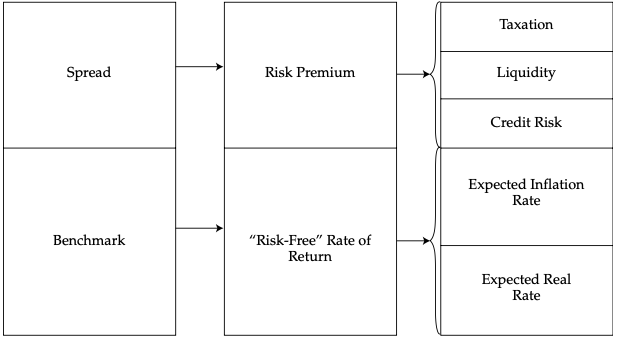
\includegraphics[scale=0.4]{/fi/yscom}
\caption{Components of Yield Spread}
\end{figure}

\begin{flushleft}
Summary of Yield Conventions
\begin{tabularx}{\textwidth}{p{11em}|X}
\hline
\rowcolor{gray!30}
Convention & Meaning \\
\hline
Actual$/$Actual & Actual number of days from prior coupon payment to settlement date/number of days in coupon period, assuming actual number of days in a year.\\
& Typically used with government bonds. \\
\hline
$30/360$ & Number of days from prior coupon payment to settlement date, assuming $30$ days in a month/number of days in a coupon period, assuming $360$ days in a year.\\
& Typically used with corporate bonds.\\
\hline
Street Convention & Yield measure that does not account for weekends and bank holidays and thus assumes cash flows are paid on their scheduled dates. \\
\hline
True Yield & Yield measure that accounts for weekends and bank holidays and thus assumes cash flows are paid after their scheduled dates. True yield is never higher than street convention yield due to the delay in time to payment.\\
\hline
Government Equiv Yield & Yield measure that restates a $30/360$ day count YTM to one based on an Actual$/$Actual day count. It is used to restate the YTM on a corporate bond to obtain the spread over the government YTM.\\
\hline
Simple Yield & Yield measure that is the sum of coupon payments plus the straight-line amortised share of the gain or loss, divided by the flat price.\\
& It is used mostly to quote Japanese government bonds (JGBs). \\
\hline
\end{tabularx}
\end{flushleft}

\begin{definition} \hlt{Annual Percentage Rate (APR)}\\
Allows conversion of an annualised yield in one periodicity to another periodicity. Compounding more frequently with lower annual rate corresponds to compounding less frequently at higher annual rate.
\begin{equation}
\left(1 + \frac{\text{APR}_m}{m} \right) = \left(1 + \frac{\text{APR}_n}{n} \right) \nonumber
\end{equation}
\end{definition}

\begin{definition} \hlt{Current Yield}\\
Measure equal to bond's annual coupon divided by flat price. Focuses solely on interest income, ignores frequency of coupon payments, interest on interest (time value of money), and accrued interest.
\begin{equation}
\text{CY}_t = \frac{\text{Annual Coupon}_t}{\text{Bond Price}_t} \nonumber
\end{equation}
\end{definition}

\begin{definition} \hlt{Simple Yield}\\
Used to quote Japanese government bonds (JGBs).
\begin{equation}
\text{Simple Yield} = \frac{1}{PV^{\text{Flat}}} \left(\sum PMT + \text{Straight Line Amortisation of Gain/Loss} \right) \nonumber
\end{equation}
\end{definition}

\begin{definition} \hlt{Bonds with Embedded Options: Yield-to-Call}\\
To modify return measure that takes bond's call feature into account.
\begin{align}
PV &= \sum\limits_{t=1}^N \frac{PMT}{(1+r)^t} + \frac{\text{Call Price}}{(1+r)^N} \nonumber \\
\text{Yield-to-Worst} &= \min\{r_i, YTM\} \nonumber
\end{align}
where $r$ is yield-to-call, to be separately calculated for each call date.\\
The \hlt{Option-Adjusted Price} is value of embedded call option added to flat price of bond. Investor bears call risk, hence embedded call option reduces value of.
\end{definition}

\begin{definition} \hlt{Option-Adjusted Yield}\\
Compute the value of the embedded option with the option pricing model, taking estimate of future interest rate volatility. Next, compute the option-adjusted price,
\begin{equation}
\text{Option-Adjusted Price} = PV^{\text{Flat}} + \text{Value of Option} \nonumber
\end{equation}
Lastly, use the option-adjusted price to compute for the yield.
\end{definition}

\begin{definition} \hlt{Bond Equivalent Yield (BEY)}\\
Periodic bond yields for straight, zero-coupon bonds computed based on semi-annual periods.\\
This yield is an internal rate of return with semi-annual compounding.
\begin{equation}
\text{BEY} = \frac{\text{Face Value} - \text{Price}}{\text{Price}} \times \frac{365}{\text{Days to Maturity}} \nonumber
\end{equation}
\end{definition}

\begin{definition} \hlt{Effective Annual Yield (EAY)}\\
Measure of return on bond if coupon payments reinvested.
\begin{equation}
\text{EAY} = \left(1 + \frac{r}{n} \right)^n - 1 \nonumber
\end{equation}
\end{definition}

\begin{remark} \hlt{BEY and EAY Relationship}\\
BEY is obtained with simple interest to annualise semi-annual YTM.
\begin{align}
\text{BEY} &= 2 \times \text{Semi-annual YTM} \nonumber \\
\text{EAY} &= \left(1 + \frac{\text{Semi-annual BEY}}{2} \right)^2 - 1 \nonumber \\
\text{BEY} &= 2(\sqrt{1+\text{EAY}} - 1) \nonumber 
\end{align}
\end{remark}

\begin{definition} Benchmark Rate Terminologies
\begin{enumerate}[label=\roman*.]
\setlength{\itemsep}{0pt}
\item On-the-Run Security: most recently issued government bond, which is also the most actively traded security and has coupon rate closest to current market discount rate. Price is close to par value.
\item Off-the-Run Security: seasoned government bonds, trade at slightly higher YTM than on-the-run bonds wth same or similar times-to-maturity, due to differences in demand for the securities and cost of financing.
\item Benchmark Spread; yield spread over a specific benchmark, represents credit risk premium, liquidity risk premium, and tax impact.
\end{enumerate}
\end{definition}

\begin{figure}[H]
\centering
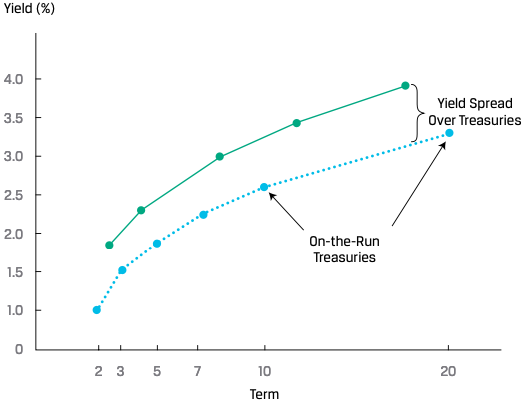
\includegraphics[scale=0.5]{/fi/otrvsotr}
\caption{On-the-run treasuries and seasoned treasuries}
\end{figure}

\begin{definition} \hlt{Government-Spread (G-Spread)}\\
Yield spread in basis points over an actual or interpolated government bond.\\
The return for bearing greater credit, liquidity, and other risks relative to the sovereign bond.
\end{definition}

\begin{method} \hlt{Approximation of G-Spread}\\
Used when comparable benchmark bond does not exist.
\begin{enumerate}[label=\roman*.]
\setlength{\itemsep}{0pt}
\item Compute the bond's current YTM
\item Linearly interpolate current rates (YTMs) for sovereign benchmark bonds with maturities closest to (below/above) given bond’s maturity, to find an approximate sovereign rate matching given bond’s maturity.
\item G-spread is difference between bond’s current YTM and interpolated sovereign benchmark rate.
\end{enumerate}
\end{method}

\begin{definition}
\label{def:ispread}
\hlt{Interpolated Spread (I-Spread)}\\
The yield spread for a bond over the standard swap rate in that currency of the same tenor.\\
Allows comparison of bonds with differing credit and liquidity risks against an interbank lending benchmark.\\
Issuers will use the I-spread to determine the relative cost of fixed-rate bonds versus floating-rate alternatives.\\
The higher the value of I-spread, the higher the compensation for liquidity and credit risk.
\end{definition}

\begin{definition} 
\label{def:zspread}
\hlt{Zero-Volatility Spread (Z-Spread)}\\
Spread added to each benchmark spot rate to make the present value of a bond’s cash flows equal its price.
\begin{align}
PV = \sum\limits_{t=1}^N \frac{PMT}{(1 + z_t + Z)^t} + \frac{FV}{(1 + z_t + Z)^N} \nonumber
\end{align}
The benchmark spot or zero rates ($z_t$) are derived from government yield curve, or from fixed rates on interest rate swaps. $Z$ is the Z-spread.
\end{definition}

\begin{definition} \hlt{Option-Adjusted Spread (OAS)}\\
Spread of fixed-income security rate and risk-free rate of return, adjusted to take into account an embedded option. Based on an option-pricing model and an assumption about future interest rate volatility.
\begin{equation}
\text{OAS} = \text{Z-Spread} - \text{Option value in basis point per year} \nonumber
\end{equation}
For callable bonds, OAS $<$ Z-Spread.
\end{definition}

\begin{flushleft}
Summary of Yield Spreads
\begin{tabularx}{\textwidth}{p{11em}|X}
\hline
\rowcolor{gray!30}
Type & Description \\
\hline
G-Spread & Yield spread in basis points over an actual or interpolated government bond.\\
& Used in the US, the UK, Japan, and other jurisdictions. \\
\hline
I-Spread & Yield spread of a bond over the standard swap rate in the same currency and with the same tenor. Euro-denominated corporate bonds are typically priced vs. a euro interest rate swap benchmark. \\
\hline
Z-Spread & A constant yield spread over a government (or interest rate swap) spot curve used to derive the term structure of credit spreads for an issuer. \\
\hline
OAS & The Z-spread adjusted for the value of an embedded call option. \\
\hline
\end{tabularx}
\end{flushleft}

\subsubsection{Yield and Yield-Spread Measures for Floating-Rate Instruments}

\begin{remark} \hlt{Floating Rate Notes Characteristics}\\
Price is constant. Principal is non-amortising and redeemed in full at maturity.\\
Reference rate determined at beginning of period, and interest payment made at end of the period (‘in arrears’).
\end{remark}

\begin{remark} \hlt{Floating Rate Notes Coupons}\\
Fluctuates as interest rates change (tied to short-term money market rate, i.e. 3 month LIBOR).\\
Coupon is dependent on reference rate and quoted margin (spread), where spread is credit related.
\end{remark}

\begin{definition} Margin Terminology
\begin{enumerate}[label=\roman*.]
\setlength{\itemsep}{0pt}
\item \hlt{Quoted Margin}: to compensate investor for differences in credit risk of issuer and that implied by reference rate. Firms with very low credit risk may be able to obtain negative quoted margin.
\item \hlt{Required Margin}: yield spread over or under reference rate such that the FRN is priced at par value on a rate reset date. This is determined by market.\\
If quoted margin equals required margin at payment date, FRN is at par.\\
If FRN is priced in between payment dates, accrued interests are quoted on Actual$/360$ or Actual$/365$.
\end{enumerate}
\end{definition}

\begin{remark} \hlt{Changes in Required Margin of Floating Rate Notes}\\
Changes in required margin come from changes in issuer’s credit risk, liquidity or tax status.\\
If credit risk dropped, then quoted margin $<$ required margin, $PV > 100$ on payment date. FRN is premium.\\
If credit risk increased, then quoted margin $<$ required margin, $PV < 100$ on payment date. FRN is discount.
\end{remark}

\begin{remark} \hlt{FRN Pull-to-Par}\\
Between payment dates, flat price will be at premium (discount) to par value if reference rate goes down (up).\\
If required margin continues to be the same as quoted margin, the flat price is pulled to par value as next reset date nears.
At reset date, any change in reference date is included in interest payment for next period.
\end{remark}

\begin{definition} \hlt{Floating Rate Notes Pricing Model}
\begin{equation}
PV = \sum\limits_{t=1}^N \frac{\frac{(MRR + QM) \times FV}{m}}{\left(1 + \frac{MRR + DM}{m} \right)^t} + \frac{FV}{\left(1 + \frac{MRR + DM}{m} \right)^N} \nonumber
\end{equation}
where $MRR$ is the market reference rate, $QM$ is quoted margin, $m$ is periodicity of floating-rate note, $DM$ is discount margin (required margin), $N$ is number of periods to maturity. Model assumes the following:
\begin{enumerate}[label=\roman*.]
\setlength{\itemsep}{0pt}
\item The $PV$ is as of rate reset date; there is no accrued interest, so the flat price is full price.
\item $30/360$ day-count convention is used, but in practice Actual$/360$ day-count is used.
\item The same $MRR$ is used for all cash flows
\end{enumerate}
\end{definition}

\subsubsection{Yield and Yield-Spread Measures for Money-Market Instruments}

\begin{remark} \hlt{Differences in Yield Measures for Money Market vs Bonds}
\begin{enumerate}[label=\roman*.]
\setlength{\itemsep}{0pt}
\item Bond YTM are annualised and compounded. Money market yields are annualised but not compounded; the return on a money market instrument is stated on a simple interest basis.
\item Bond YTM are stated on a common periodicity for all times-to-maturity. Money market instruments with different times-to-maturity have different periodicities for the annual rate.
\item Bond YTM can be calculated using standard time-value-of-money analysis. Money market instruments are often quoted using non-standard interest rates and require different pricing equations.
\end{enumerate}
\end{remark}

\begin{method} \hlt{Discount-Rate Pricing}
\begin{equation}
PV = FV \times \left(1 - \frac{\text{Days}}{\text{Years}}\times DR \right) \nonumber
\end{equation}
where $DR$ is the discount rate stated in annual percentage rate. Equation may be rewritten as
\begin{equation}
DR = \frac{\text{Days}}{\text{Years}} \times \frac{(FV-PV)}{FV} \nonumber
\end{equation}
where the first term is periodicity of the annual rate. Note that the discount rate understates rate of return to investor, and understates cost of borrowed funds to issuer.\\
The quoted amount is $FV$, for commercial paper, treasury bills, banker's acceptances.
\end{method}

\begin{method} \hlt{Add-On Rate Pricing}
\begin{equation}
PV = \frac{FV}{\left( 1 +  \frac{\text{Days}}{\text{Years}} \times AOR \right)} \nonumber
\end{equation}
where $AOR$ is the add-on-rate in annual percentage term. Equation may be rewritten as
\begin{equation}
AOR = \frac{\text{Days}}{\text{Years}} \times \frac{(FV-PV)}{PV} \nonumber 
\end{equation}
First term is the periodicity, and second term is return on investment.\\
The quoted amount is $PV$, for bank certificates of deposit, repurchase agreements (Repos), MRRs.
\end{method}

\begin{method} \hlt{Comparing Money Market Instruments on Bond Equivalent Yield Basis}
\begin{enumerate}[label=\roman*.]
\setlength{\itemsep}{0pt}
\item For a MM instrument quoted on DR basis, determine price per 100 of Par (PV).
\item Determine AOR for this MM instrument using PV.
\item Bond Equivalent Yield (BEY) is a MM rate stated on a $365$-day AOR basis. This instrument is now comparable with other MM instruments expressed on a BEY basis.
\end{enumerate}
\end{method}

\subsubsection{Arbitrage-Free Valuation Framework}

\begin{definition} \hlt{Value Additivity Arbitrage}\\
Value of the whole differs from the sum of value of parts.
\begin{enumerate}[label=\roman*.]
\setlength{\itemsep}{0pt}
\item Stripping: portfolio of strips trading less than intact bond. To purchase the strips, combine them, then sell them as a bond.
\item Reconstitution: bond is worth less than its components. To purchase the bond, break it into portfolio of strips, then sell the components.
\end{enumerate}
\end{definition}

\begin{definition} \hlt{Dominance Arbitrage}\\
One asset trades at lower price than another asset with identical characteristics.
\end{definition}

\begin{figure}[H]
\centering
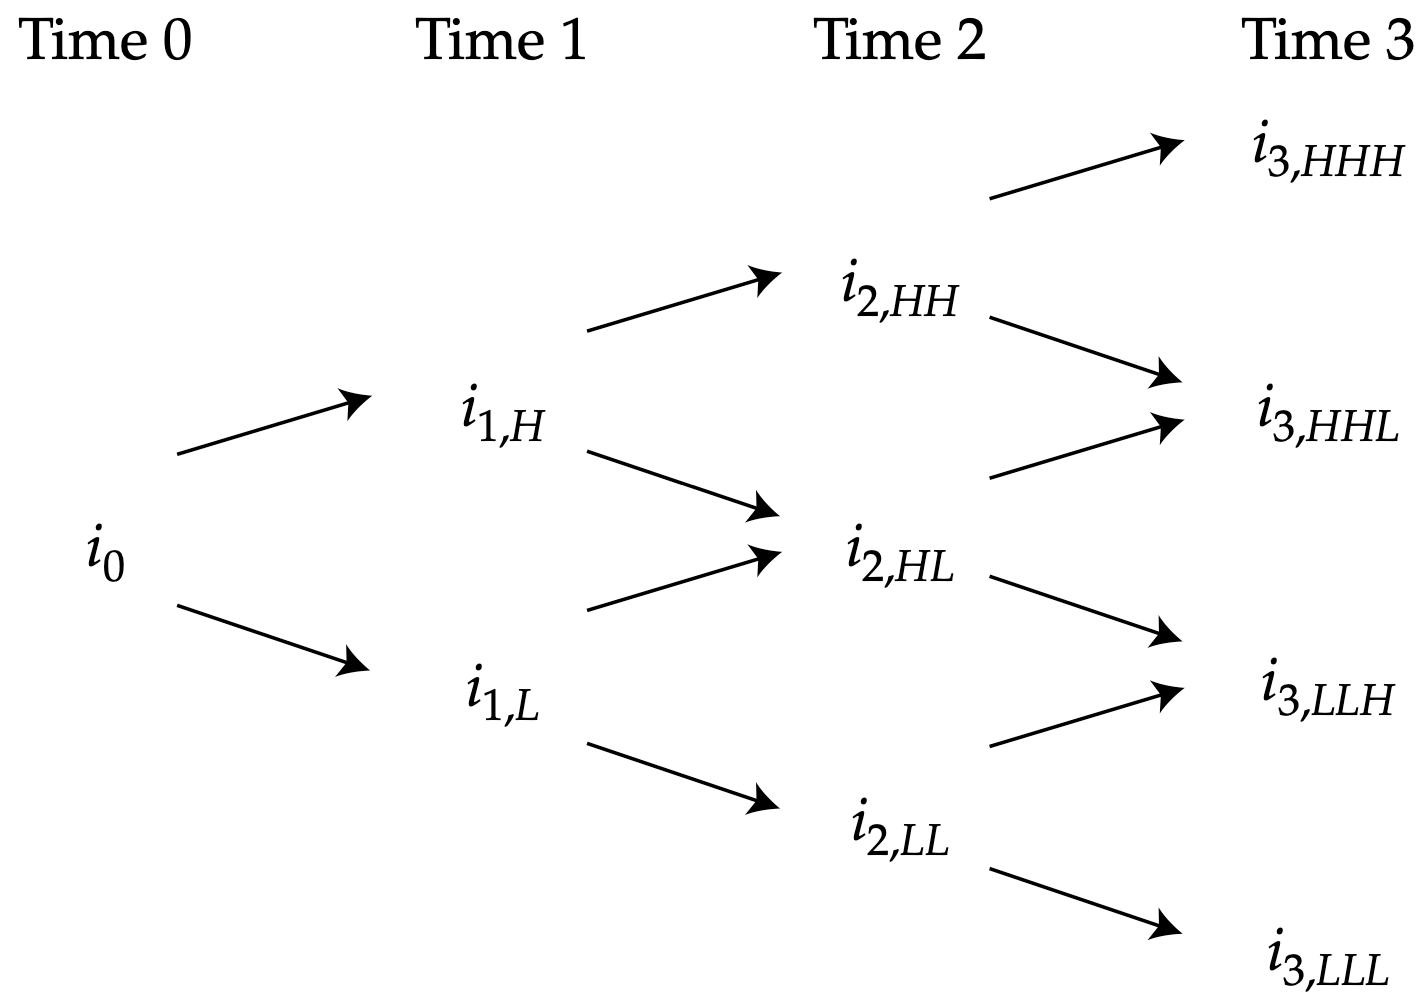
\includegraphics[scale=0.25]{/fi/bintree}
\caption{Binomial interest rate tree}
\end{figure}

\begin{method} \hlt{Binomial Interest Rate Tree}\\
Assumes interest rates have equal probability of taking one of two possible values in the next period.\\
Starting point $i_0$ of tree is current $1$-period spot rate.\\
A lognormal random walk is assumed for the implied interest rate, as lognormal properties allows for non-negativity of interest rates and higher volatility at higher interest rates. Note that
\begin{equation}
i_{1, H} = i_{i,L} e^{2 \sigma} \nonumber
\end{equation}
where $\sigma$ is the standard deviation of interest rates. Two vertical-adjacent nodes differ by factor of $e^{2 \sigma}$.
\end{method}

\begin{figure}[H]
\centering
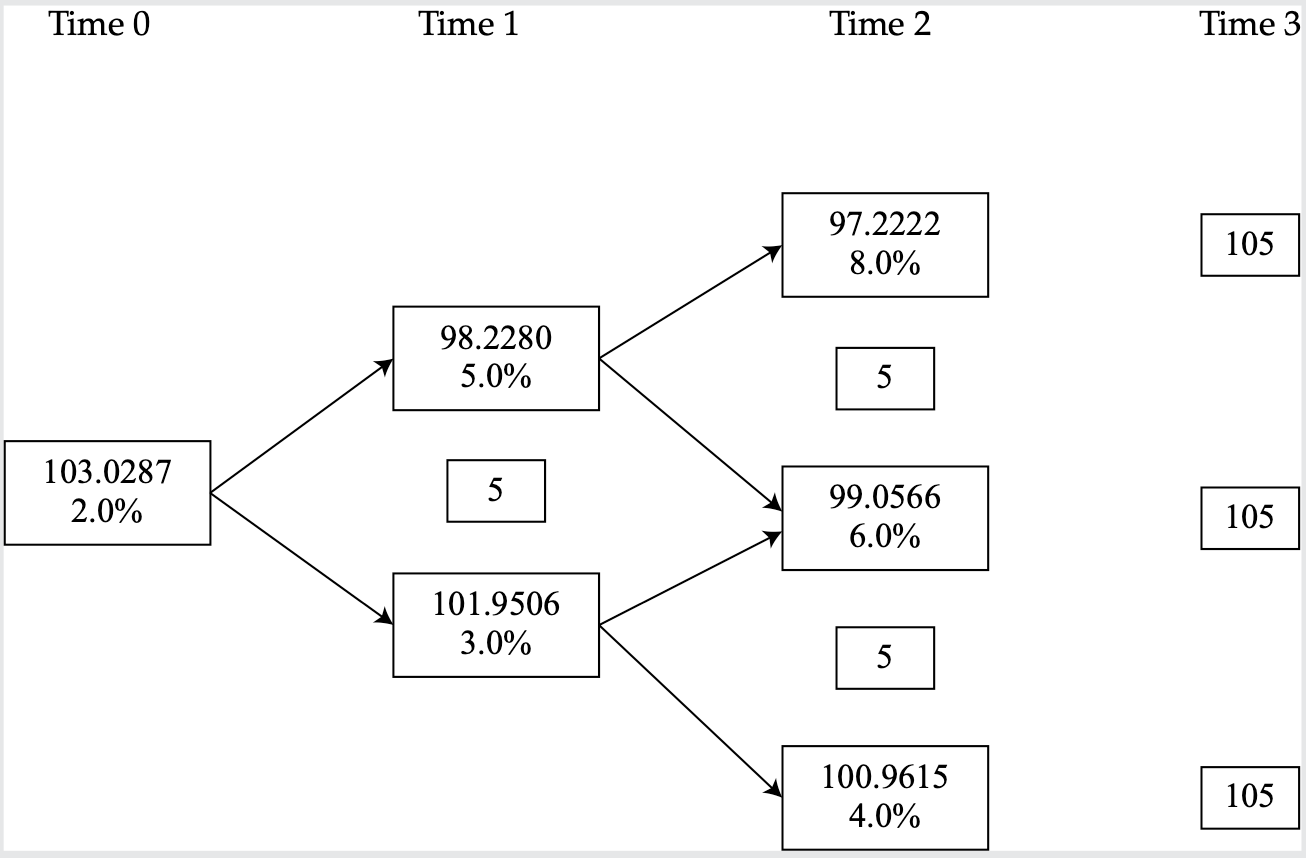
\includegraphics[scale=0.4]{/fi/backwardinduc}
\caption{Backward induction of binomial tree}
\end{figure}

\begin{method} \hlt{Backward Induction of Binomial Tree for Straight Bonds}\\
for $t$ in range $(0, T-1, -1)$: \# Computing from second last layer to the first \\
{\color{white}space} for $n$ in layer$\_t\_$nodes:
\begin{equation}
\text{v}(t,n) = \frac{\text{PMT}(t+1,n)+ [0.5 \text{v}(t+1, nH) + 0.5 \text{v}(t+1, nL)]}{1 + i(t, n)} \nonumber
\end{equation}
where $\text{v}(t,n)$ is value of node at time $t$ at position $n$, $\text{v}(t+1,nH)$ and $\text{v}(t+1,nL)$ is value of node at next time step $t+1$ at positions up ($H$) and down ($L$), $\text{PMT}(t+1,n)$ is beginning coupon payment for next time step, $i(t,n)$ is interest rate at time $t$ at position $n$ in decimal. \\
Note that at last layer $T$, the value at node $n$ is as follows:
\begin{equation}
\text{v}(T, n) = \frac{\text{PMT}(T,n) + \text{Redemption Value}(T,n)}{1 + i(T, n)} \nonumber
\end{equation}
\end{method}

\begin{remark} \hlt{Calibration of Software for Binomial Tree}
\begin{enumerate}[label=\roman*.]
\setlength{\itemsep}{0pt}
\item Interest rate tree should generated arbitrage-free values for benchmark security. Value of bonds produced by tree much be equal to their market pice.
\item Vertically-adjacent rates are $e^{2 \sigma}$ values apart
\item The middle forward rate in a period is approximately equal to the implied (from benchmark spot rate curve) one-period forward rate for that period
\end{enumerate}
\end{remark}

\begin{method} \hlt{Path-Wise Valuation}
\begin{enumerate}[label=\roman*.]
\setlength{\itemsep}{0pt}
\item Specify list of all potential paths along the tree
\item Determine the present value of a bond along each potential path
\item Calculate the average across all possible paths.
\end{enumerate}
\end{method}

\begin{method} \hlt{Monte Carlo Simulation}
\begin{enumerate}[label=\roman*.]
\setlength{\itemsep}{0pt}
\item Simulate numerous paths of interest rates under a volatility assumption and probability distribution
\item Generate spot rates from the simulated interest rates
\item Calculate present value from the cash flow along each interest rate path
\item Take the average of the present value across all interest rate paths
\end{enumerate}
Simulated paths should be calibrated so benchmark interest rate paths value benchmark securities at market price (arbitrage-free valuation). Calibration process involves adding/subtracting a constant to all rates when value from simulated paths is too high/low relative to market prices. This will result in a drift adjusted model.\\
Upper and lower bounds on interest rates may be imposed; bounds are based on notion of mean reversion.
\end{method}

\subsubsection{Valuation of Bonds with Embedded Options}

\begin{remark} \hlt{Embedded Options}\\
Allows issuer to manage interest rate risk, and/or issue bonds at an attractive coupon rate.
\end{remark}

\begin{remark} \hlt{Types of Bond Options}
\begin{enumerate}[label=\roman*.]
\setlength{\itemsep}{0pt}
\item Callable bond: gives issuer option to call back the bond. Investor is short the option.\\
Callable bonds usually have call protection period in which the bond cannot be called.
\item Putable bond: allows investor to put the bond back to issuer prior to maturity. Investor is long put.
\item Extendible bond: allows investor to extend maturity of bond.\\
May be evaluated as a putable bond with longer maturity.
\item Estate put: includes provision that allows heirs of investor to put the bond back to issuer upon death of investor. Value of contingent put option is inversely the investor's life expectancy.
\item Sinking fund bonds: require issuer to set aside funds periodically to retire the bond.\\
Reduces the credit risk of the bond over time. Sinkers typically have several related issuer options (call provisions, acceleration provisions, delivery options).
\end{enumerate}
\end{remark}

\begin{remark} \hlt{Value of Callable Bonds}\\
Investor is long bond but short the call option. Value of call option decreases the value of the callable bond.
\begin{equation}
v_{\text{Call Option}} = v_{\text{Straight Bond}} - v_{\text{Callable Bond}} \nonumber
\end{equation}
\end{remark}

\begin{remark} \hlt{Value of Putable Bonds}\\
Investor is long both bond and putable option. Value of put option increases the value of putable bond.
\begin{equation}
v_{\text{Put Option}} = v_{\text{Putable Bond}} - v_{\text{Straight Bond}} \nonumber
\end{equation}
\end{remark}

\begin{remark} \hlt{Interest Rate Volatility on Value of Callable or Putable Bond}\\
If interest rate volatility increases, values of both call and put options increase, hence value of callable bond decreases, while value of putable bond increases.
\end{remark}

\begin{figure}[H]
\centering
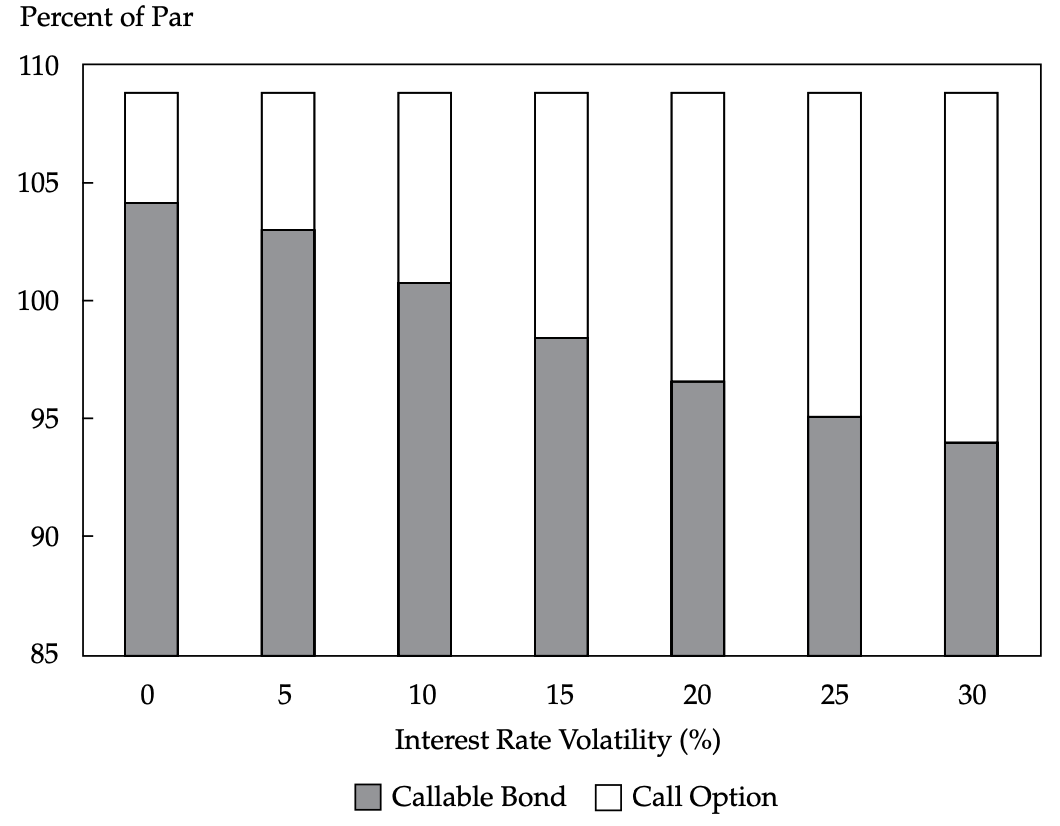
\includegraphics[scale=0.35]{/fi/volchangecallbond}
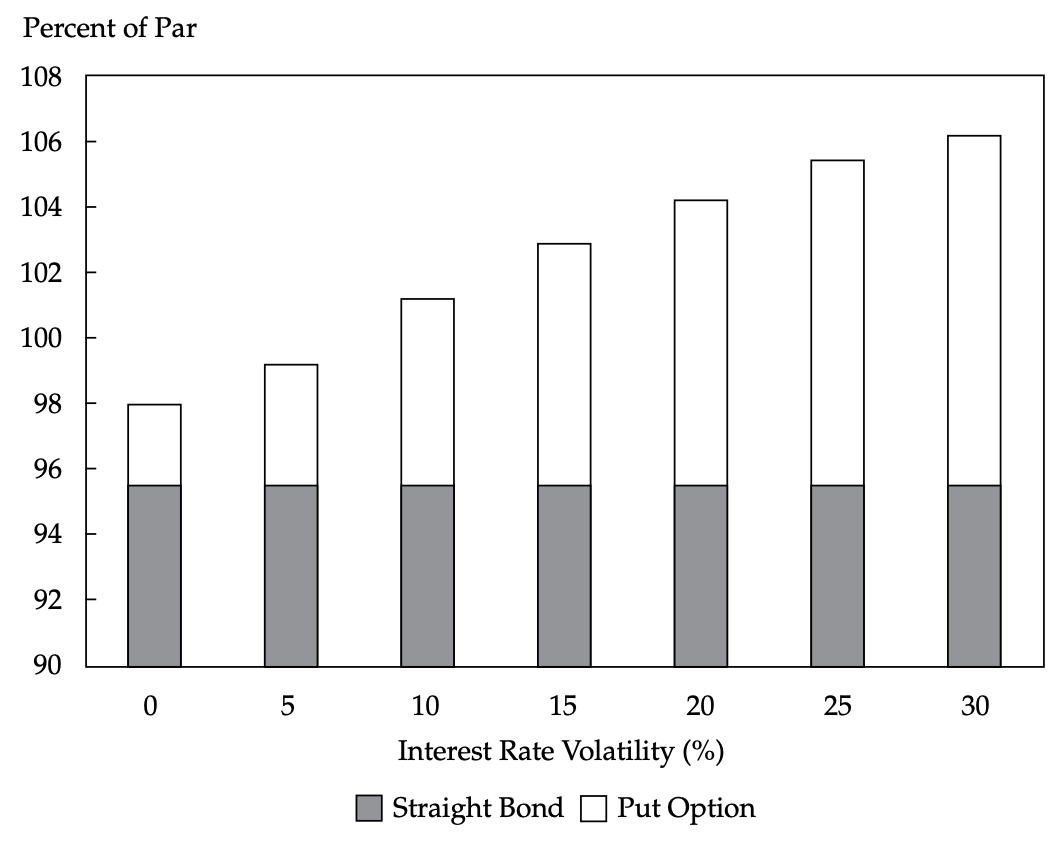
\includegraphics[scale=0.35]{/fi/volchangeputbond}
\caption{Effect of change in interest rate volatility on value of callable and putable bonds}
\end{figure}

\begin{remark} \hlt{Interest Rate Level on Value of Callable or Putable Bond}\\
As interest rates decrease, short call in callable bond limits bond's upside, hence value of callable bond rises less rapidly than value of otherwise equivalent straight bond.\\
As interest rtes increase, long put in putable bond hedges against loss in value, hence value of putable bond falls less rapidly than value of otherwise equivalent straight bond.\\
Call option value is inversely correlated to level of interest rates.\\
Put option is directly correlated to level of interest rates.
\end{remark}

\begin{figure}[H]
\centering
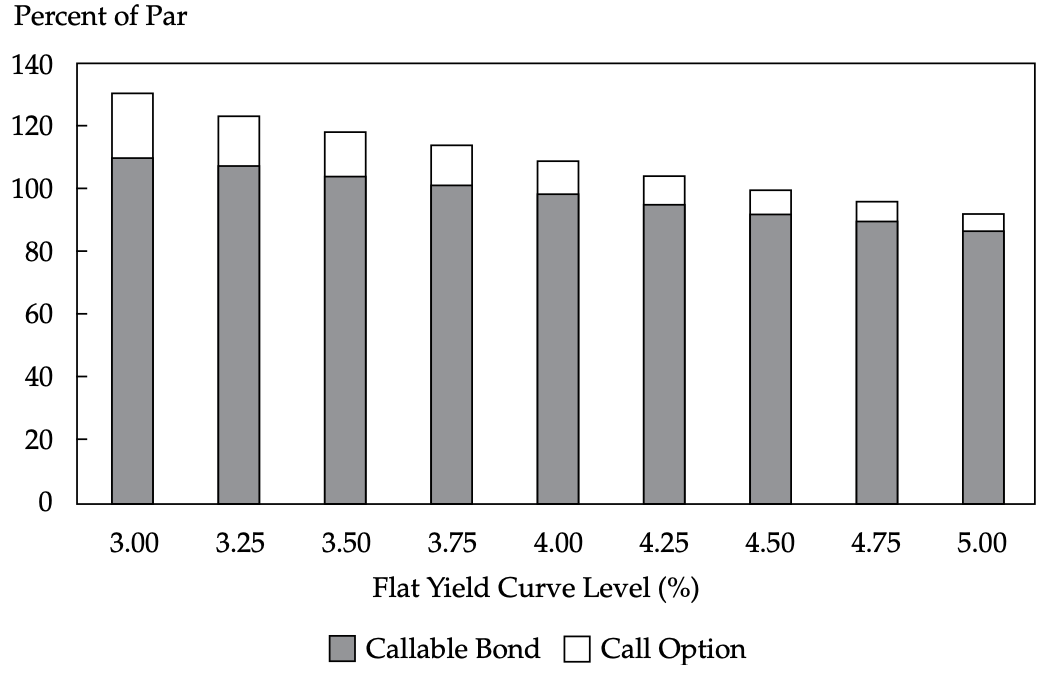
\includegraphics[scale=0.44]{/fi/flatyieldcurvelvcallbond}
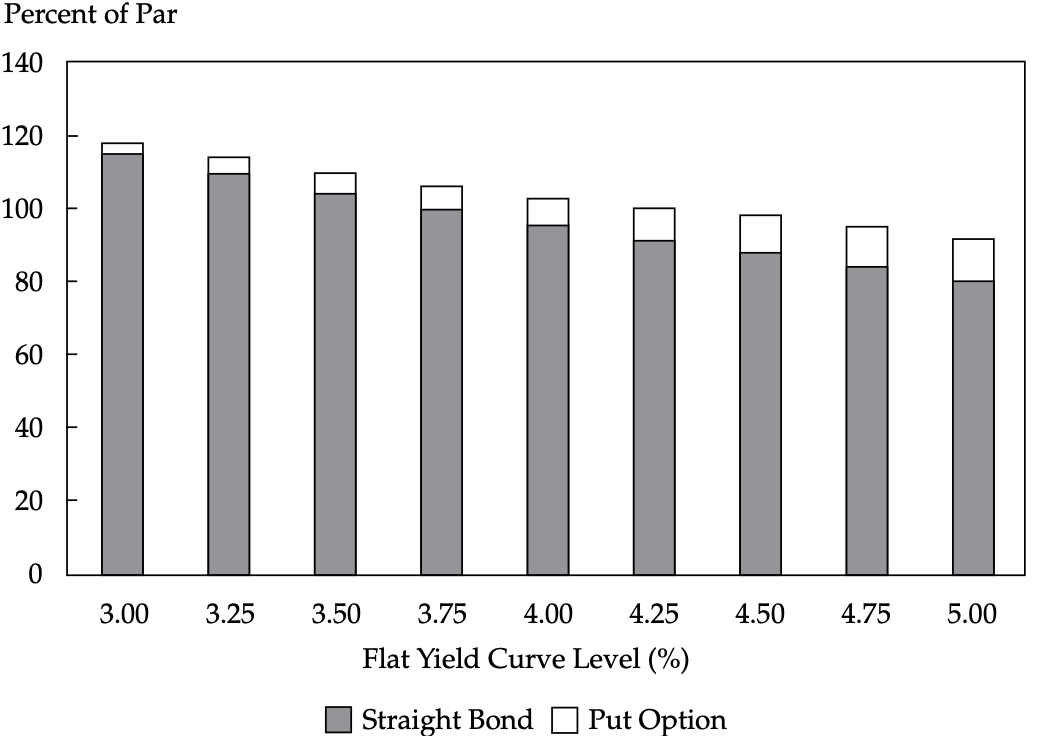
\includegraphics[scale=0.4]{/fi/flatyieldcurvelvputbond}
\caption{Value of callable and putable bond under different flat yield curve levels}
\end{figure}

\begin{remark} \hlt{Yield Curve Shape on Value of Callable or Putable Bond}\\
Value of embedded call option increases as interest rates decline.\\
When yield curve is upward sloping, distant one-period forward rates are higher than near one-period forward rates. Higher interest rate scenario limits probability of call option bing in the money, hence value of call option will be lower for upward sloping yield curve. As upward-sloping yield curve flattens, call option value increases.\\
Value of put option increases with interest rates. Upward sloping yield curve indicates higher probability of put option going in the money. Put option value declines as yield curve flattens.
\end{remark}

\begin{figure}[H]
\centering
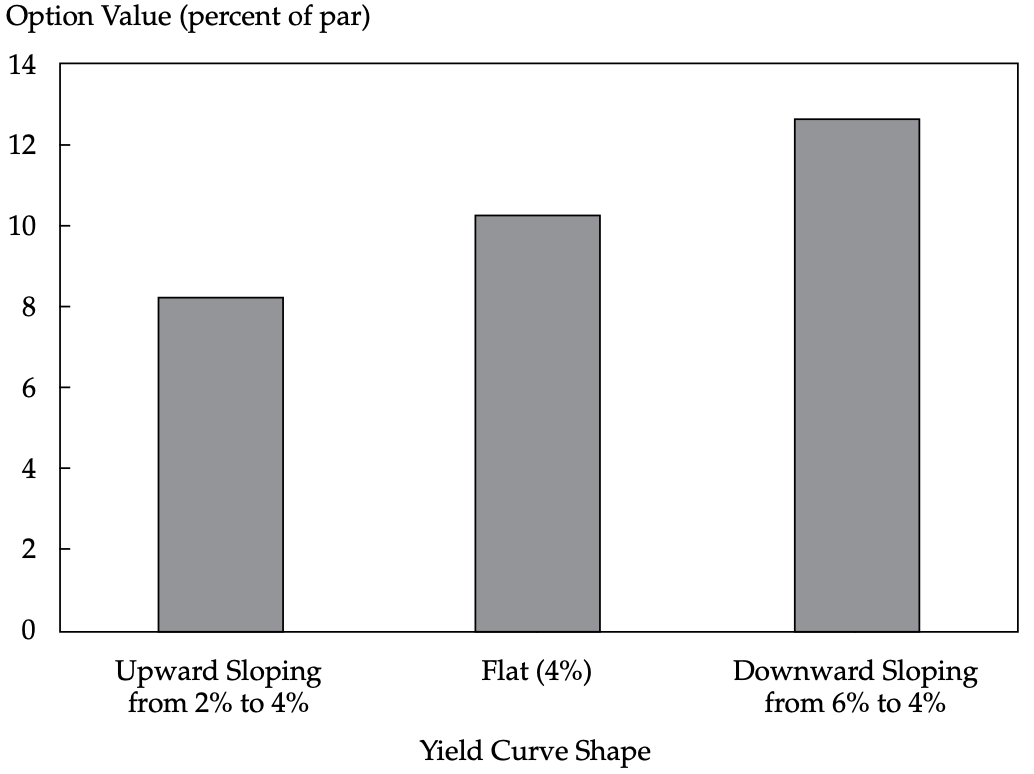
\includegraphics[scale=0.35]{/fi/yieldcurveshapecallbond}
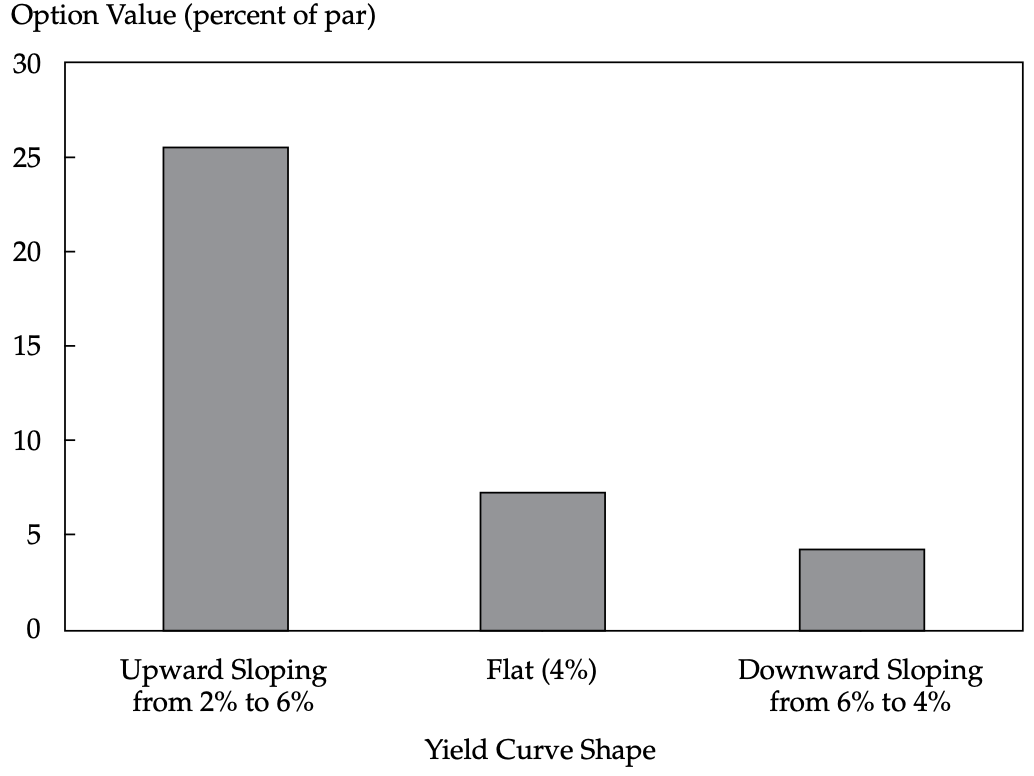
\includegraphics[scale=0.35]{/fi/yieldcurveshapeputbond}
\caption{Value of putable bond under different flat yield curve shapes}
\end{figure}

\begin{method} \hlt{Backward Induction of Binomial Tree for Bonds with Embedded Options}\\
One-period forward rates are used, instead of spot rates.\\
for $t$ in range $(0, T-1, -1)$: \# Computing from second last layer to the first \\
{\color{white}space} for $n$ in layer$\_t\_$nodes:
\begin{align}
\text{v}(t,n) = \frac{\text{PMT}(t+1,n)+ [0.5 \text{v}(t+1, nH) + 0.5 \text{v}(t+1, nL)]}{1 + i(t, n)} \nonumber
\end{align}
{\color{white}space} {\color{white}space} if option is callable:
\begin{equation}
\text{v}(t,n) = \min \{\text{Strike}, \text{v}(t,n) \} \nonumber
\end{equation}
{\color{white}space} {\color{white}space} if option is putable:
\begin{equation}
\text{v}(t,n) = \max \{\text{Strike}, \text{v}(t,n) \} \nonumber
\end{equation}
where $\text{v}(t,n)$ is value of node at time $t$ at position $n$, $\text{v}(t+1,nH)$ and $\text{v}(t+1,nL)$ is value of node at next time step $t+1$ at positions up ($H$) and down ($L$), $\text{PMT}(t+1,n)$ is beginning coupon payment for next time step, $i(t,n)$ is interest rate at time $t$ at position $n$ in decimal. \\
Note that at last layer $T$, the value at node $n$ is as follows:
\begin{equation}
\text{v}(T, n) = \frac{\text{PMT}(T,n) + \text{Redemption Value}(T,n)}{1 + i(T, n)} \nonumber
\end{equation}
\end{method}

\begin{figure}[H]
\centering
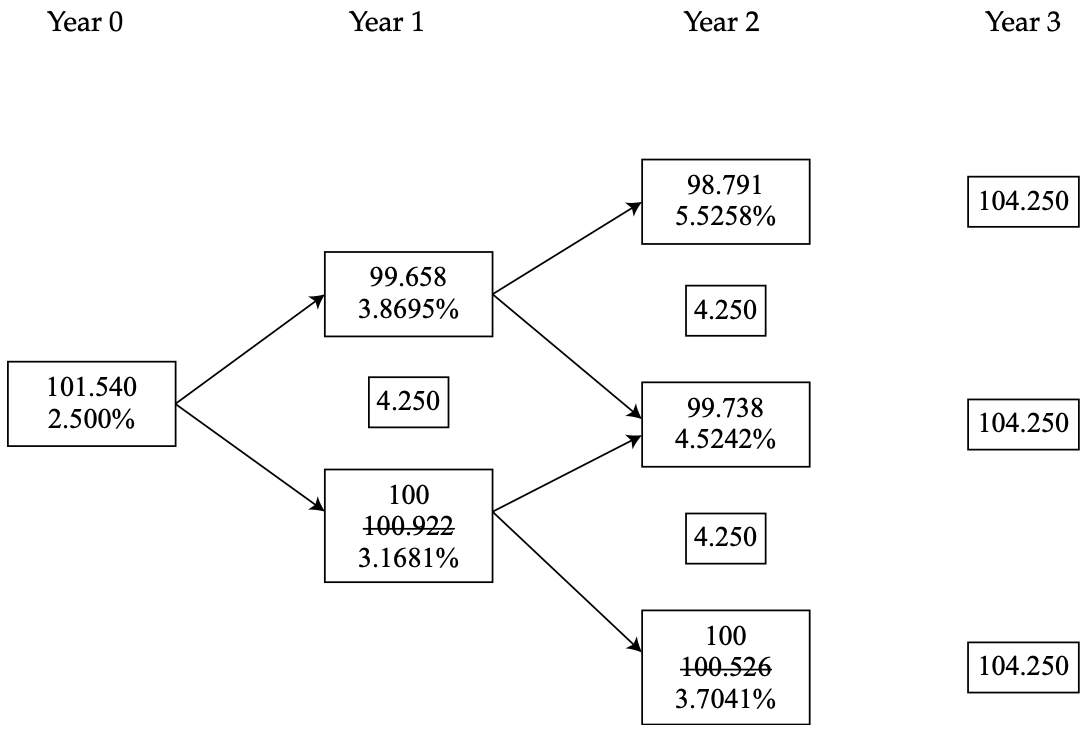
\includegraphics[scale=0.4]{/fi/backwardinduccallable}
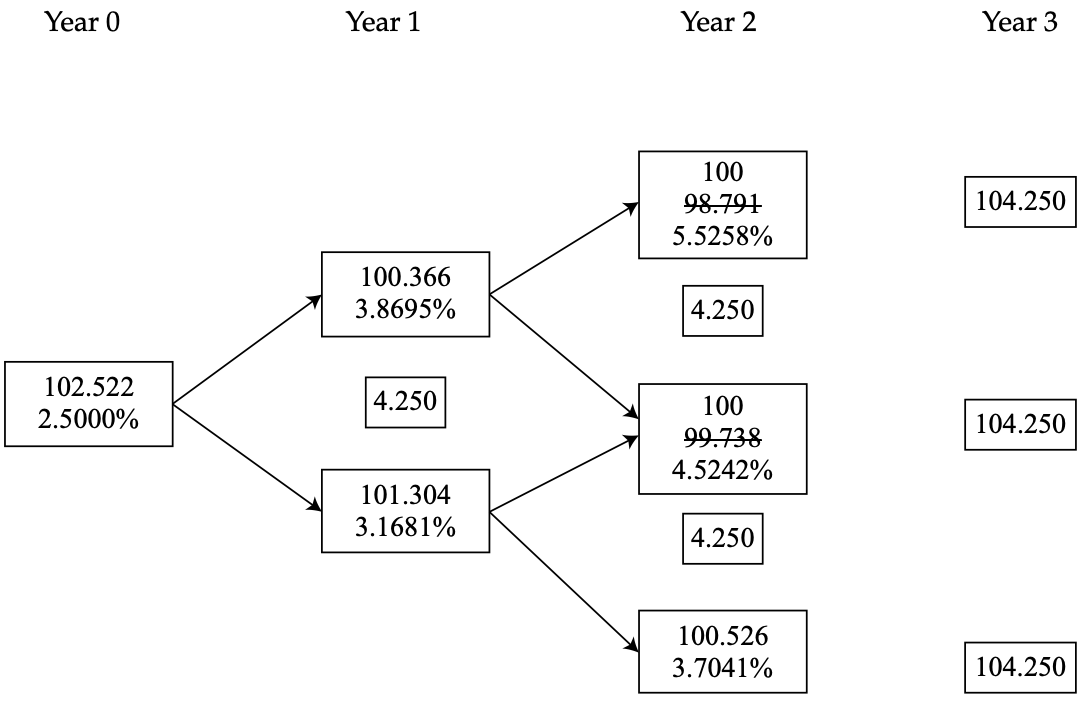
\includegraphics[scale=0.4]{/fi/backwardinducputable}
\caption{Backward induction with adjustment of node values for callable and putable bonds}
\end{figure}

\begin{remark} \hlt{Option-Adjusted Spreads (OAS) for Risky Callable and Putable Bonds}\\
Constant spread added to all one-period rates in the tree such that the calculated value equals market price. This spread is only added to the tree after adjustment for the embedded option.\\
If OAS for a bond is higher than OAS of its peers for the same credit risk, it is undervalued, vice versa.
\end{remark}

\begin{figure}[H]
\centering
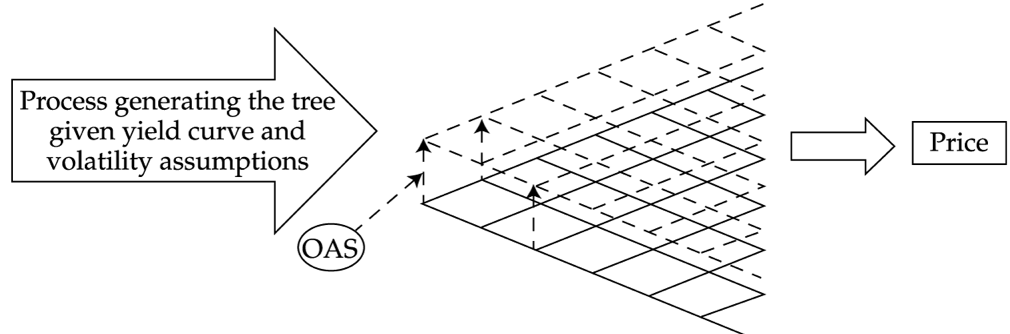
\includegraphics[scale=0.5]{/fi/oas}
\caption{Option-adjusted spread}
\end{figure}

\begin{remark} \hlt{Interest Rate Volatility on OAS}\\
Higher volatility lead to increased value of call option, hence decreasing the value of the call option. Hence when estimated volatility of benchmark rates used is higher, the computed value of callable bond will be lower, hence close to its true market price. The OAS that needs to be added to benchmark rates to correctly price the bond is therefore lower.\\
Hence, as assumed level of volatility used in interest rate tree increases, the computed OAS for a callable bond decreases. The computed OAS for a putable bond increases as the assumed level of volatility increases.
\end{remark}

\begin{flushleft}
Relationship Between Volatility and OAS
\begin{tabularx}{\textwidth}{p{5em}|X|X|X|X|X|X}
\hline
\rowcolor{gray!30}
Volatility & Call & Put & Callable & Putable & OAS$_{\text{Call}}$ & OAS$_{\text{Put}}$ \\
\hline
High & High & High & Low & High & Low & High \\
\hline
Low & Low & Low & High & Low & High & Low \\
\hline
\end{tabularx}
\end{flushleft}

\begin{figure}[H]
\centering
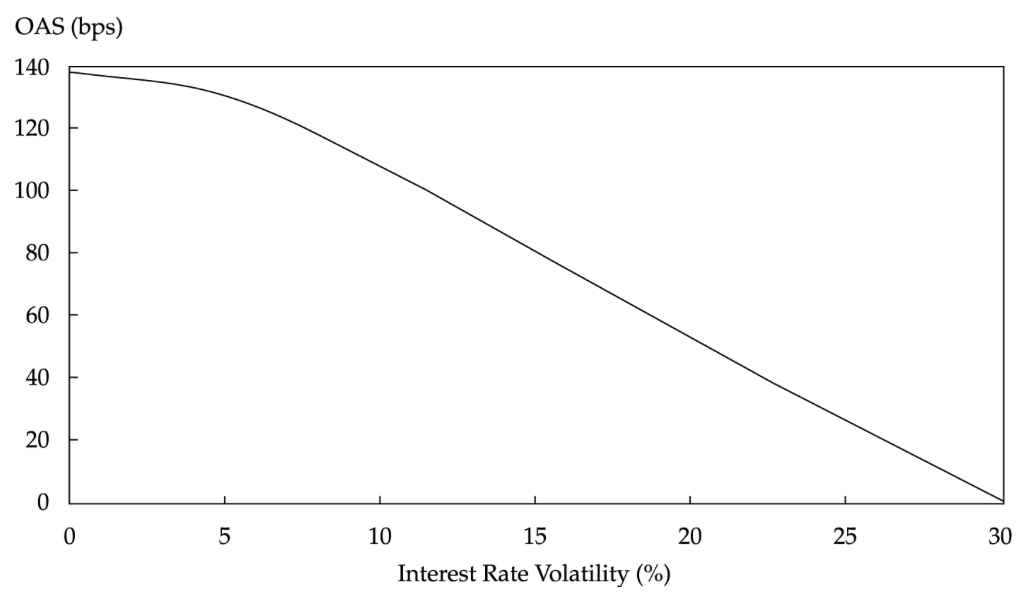
\includegraphics[scale=0.45]{/fi/voloas}
\caption{Interest rate volatility on OAS for a callable bond}
\end{figure}

\begin{remark} \hlt{Value of Floored Floater}\\
Capped floater protects investor against declining interest rates, hence is an investor option.\\
Investor is long bond long option, hence value of floor increases value of floored floater relative to straight bond.
\begin{equation}
v_{\text{Floored Floater}} = v_{\text{Straight Bond}} + v_{\text{Embedded Floor}} \nonumber
\end{equation}
\end{remark}

\begin{remark} \hlt{Value of Capped Floater}\\
Capped floater protects issuer against rising interest rates, hence is an issuer option.\\
Investor is long bond short option, hence value of cap decreases value of capped floater relative to straight bond.
\begin{equation}
v_{\text{Capped Floater}} = v_{\text{Straight Bond}} - v_{\text{Embedded Cap}} \nonumber
\end{equation}
\end{remark}

\begin{method} \hlt{Backward Induction of Binomial Tree for Floored Floater and Capped Floater}\\
One-period forward rates are used, instead of spot rates. \\
for $t$ in range $(0, T-1, -1)$: \# Computing from second last layer to the first \\
{\color{white}space} for $n$ in layer$\_t\_$nodes: \\
{\color{white}space} {\color{white}space} if option is floored floater:
\begin{equation}
\text{PMT}(t,n) = \min \{\text{Min Interest Rate} \times 100, \text{Coupon Rate} \times 100\} \nonumber
\end{equation}
{\color{white}space} {\color{white}space} if option is capped floater:
\begin{equation}
\text{PMT}(t,n) = \max \{\text{Min Interest Rate} \times 100, \text{Coupon Rate} \times 100\} \nonumber
\end{equation}
{\color{white}space} Then compute value:
\begin{align}
\text{v}(t,n) = \frac{\text{PMT}(t+1,n)+ [0.5 \text{v}(t+1, nH) + 0.5 \text{v}(t+1, nL)]}{1 + i(t, n)} \nonumber
\end{align}
where $\text{v}(t,n)$ is value of node at time $t$ at position $n$, $\text{v}(t+1,nH)$ and $\text{v}(t+1,nL)$ is value of node at next time step $t+1$ at positions up ($H$) and down ($L$), $\text{PMT}(t+1,n)$ is beginning coupon payment for next time step, $i(t,n)$ is interest rate at time $t$ at position $n$ in decimal. \\
Note that at last layer $T$, the value at node $n$ is as follows:
\begin{equation}
\text{v}(T, n) = \frac{\text{PMT}(T,n) + \text{Redemption Value}(T,n)}{1 + i(T, n)} \nonumber
\end{equation}
Redemption value to be computed using the floored or capped floater PMT computation earlier.
\end{method}

\begin{figure}[H]
\centering
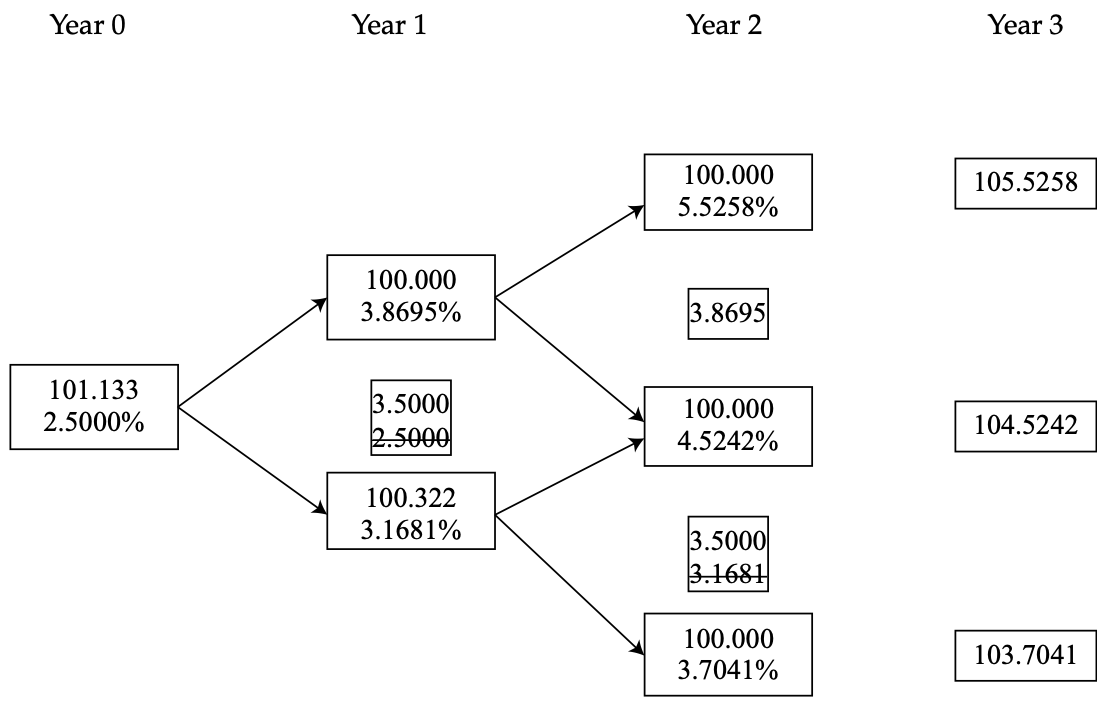
\includegraphics[scale=0.4]{/fi/backwardinducfloor}
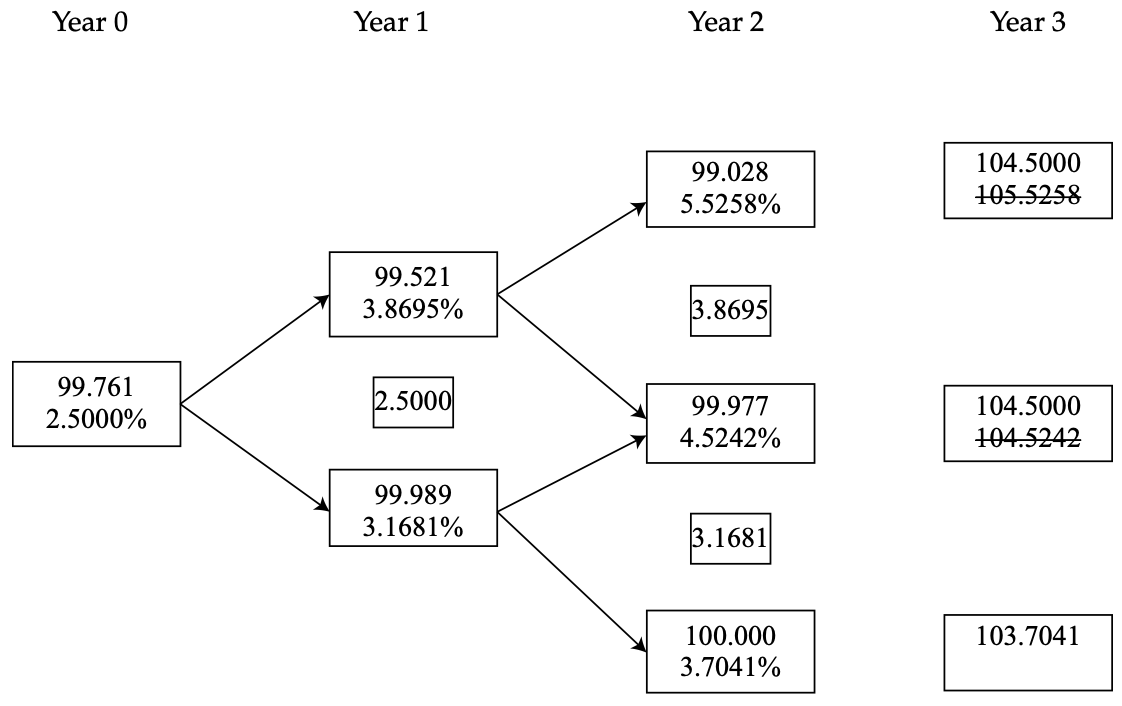
\includegraphics[scale=0.4]{/fi/backwardinduccap}
\caption{Backward induction with adjustment of node values for floor and cap floater bonds}
\end{figure}

\begin{remark} \hlt{Convertible Bonds}\\
Investor has right to convert the bond into fixed number of shares during the conversion period at conversion price, hence enjoying the upside of the issuer stock at cost of lower yield. Existing shareholders face dilution.\\
Offer document will indicate how the initial conversion ratio would be modified to account for corporate actions such as stock splits or stock dividends. \\
Offer documents may provide contingent put option in event of change-of-control events such as mergers; this may be exercised for a specific period of time after change of control. Alternatively, a lower conversion price may be specified in event of change of control. Conversion ratio may be adjusted upward if company pays dividend in excess of specified threshold dividend, hence protecting bondholders in event that the company pays out an unusually large dividend, which cause the ex-dividend price of stock to decline.\\
Other put options such as hard puts (i.e., redeemable for cash) or soft puts (i.e., issuer decides whether to redeem the bond for cash, stock, subordinated debentures, or combination of the three) may be embedded.
\end{remark}

\begin{remark} Convertible Bonds Terminology
\begin{enumerate}[label=\roman*.]
\setlength{\itemsep}{0pt}
\item \hlt{Conversion Value}: value of common stock that the bond maybe converted.
\begin{equation}
\text{Conversion Value} = \text{Market Price of Stock} \times \text{Conversion Ratio} \nonumber
\end{equation}
\item \hlt{Straight/Investment Value}: value of convertible bond if it were not convertible
\item \hlt{Minimum Value}: greater of its conversion value or straight value.\\
If convertible bond sells for less than its conversion value, then it could be purchased, immediately converted into common stock, and the stock sold for more than cost of the bond.
\item \hlt{Market Conversion Price/Conversion Parity Price}: price that convertible bondholder would pay for the stock if the bond is bought and immediately converted.
\begin{equation}
\text{Market Conversion Price} = \frac{\text{Market Price of Convertible Bond}}{\text{Conversion Ratio}} \nonumber
\end{equation}
\item \hlt{Market Conversion Premium Per Share}: market conversion price minus current market price.
\begin{equation}
\text{Market Conversion Premium Ratio} = \frac{\text{Market Conversion Premium per Share}}{\text{Market Price of Common Stock}} \nonumber
\end{equation}
\item \hlt{Premium Over Straight Value}: measure of downside risk, which is limited by bond's underlying straight value as price of convertible bond will not fall below this value.\\
The greater the premium over straight value, the less attractive the convertible bond.\\
Straight value is not constant, and varies with changes in interest rate and credit spread of bond.
\begin{equation}
\text{Premium Over Straight Value} = \frac{\text{Convertible Bond Price}}{\text{Straight Value}} - 1 \nonumber
\end{equation}
\end{enumerate}
\end{remark}

\begin{remark} \hlt{Contingent Convertibles}
\begin{enumerate}[label=\roman*.]
\setlength{\itemsep}{0pt}
\item Contingent Convertible Bonds ('CoCos'): pay higher coupon than otherwise identical non-convertible bonds, but are deeply subordinated and may be converted into equity or face principal write-downs if regulatory capital ratios are breached.
\item Convertible Contingent Convertible Bonds ('CoCoCos'): combined traditional convertible bond and a 'CoCo'. Convertible at discretion of investor, hence offering upside potential if share price increases. Also converted into equity or face principal write-downs in event of regulatory capital breach.
\end{enumerate}
\end{remark}

\begin{remark} \hlt{Value of Convertible Bonds in Arbitrage-Free Framework}\\
Investing in non-callable/non-putable convertible bond is equivalent to buying an option-free bond and a call option on amount of common stock equal to conversion ratio.
\begin{enumerate}[label=\roman*.]
\setlength{\itemsep}{0pt}
\item Non-Callable/Non-Putable Convertible Bond
\begin{equation}
\text{Bond Value} = \text{Straight Value} + \text{Call Option on Stock} \nonumber
\end{equation}
\item Callable Convertible Bond: includes call option that gives issuer right to call the bond
\begin{equation}
\text{Bond Value} = \text{Straight Value} + \text{Call Option on Stock} - \text{Call Option on Bond} \nonumber
\end{equation}
\item Convertible Bond that is Callable and Putable
\begin{equation}
\text{Bond Value} = \text{Straight Value} + \text{Call Option on Stock} - \text{Call Option on Bond} + \text{Put Option on Bond} \nonumber
\end{equation}
\end{enumerate}
\end{remark}

\begin{remark} \hlt{Difficulties of Valuing Convertible Bonds}\\
More difficult to value than callable bonds. To consider all of the factors that affect the value of callable bond, including interest rates and interest rate volatility, plus all of the factors that affect issuer’s common stock price and options on its common stock, such as its price volatility.
\end{remark}

\begin{remark} \hlt{Characteristics of Underlying Stock Price and Risk-Return of Convertible Bond}
\begin{enumerate}[label=\roman*.]
\setlength{\itemsep}{0pt}
\item If stock price falls, return on convertible bonds exceed those of the stock, as convertible bond's price has floor equal to straight bond value. As stock price approaches zero, convertible value will move towards the present value of estimated recovery.
\item If stock price rises, bond will underperform due to conversion premium.
\item If stock price is stable, return on convertible bond may exceed stock return due to coupon payments received from the bond, assuming no change in interest rates or credit risk of issuer.
\item If stock price is so low that it has little or no effect on convertible's price, bond trades as though it is a straight bond, and is referred to as a busted convertible.
\item If stock price is so high that convertible behaves as though it is an equity, the convertible is a common stock equivalent.
\end{enumerate}
\end{remark}

\begin{figure}[H]
\centering
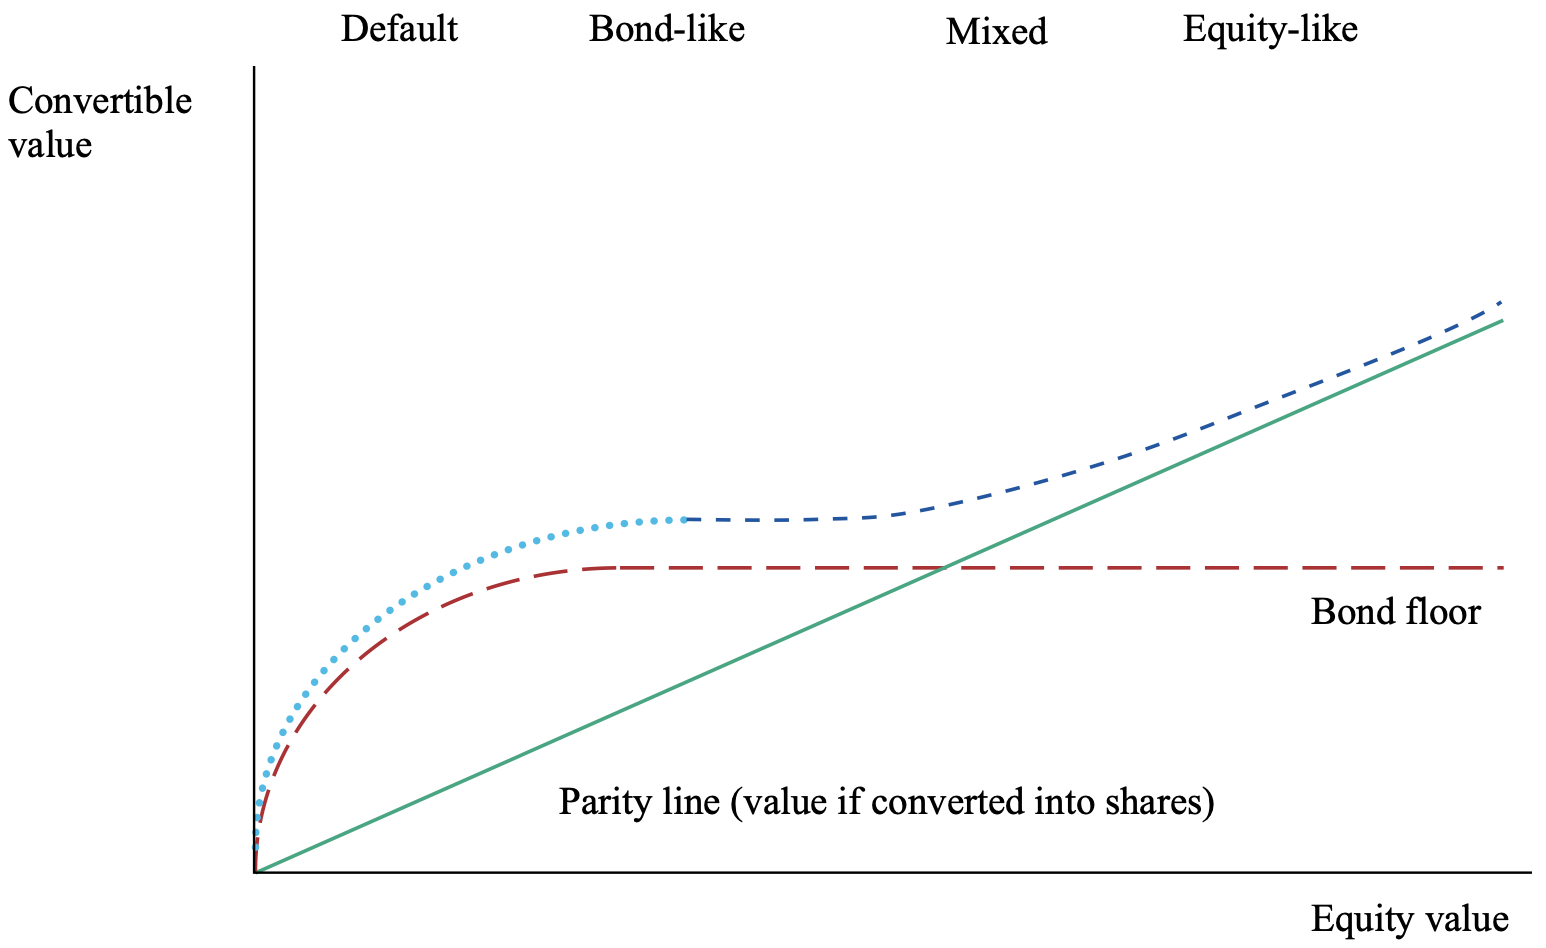
\includegraphics[scale=0.4]{/fi/convertiblebehavior}
\caption{Price behaviour of convertible bond and underlying common stock}
\end{figure}